\documentclass{article}
\usepackage[utf8]{inputenc}
\usepackage{amsfonts, amsmath, fullpage, natbib, graphicx}

\usepackage{subcaption}
\usepackage[margin=.75in]{geometry}
\usepackage[dvipsnames]{xcolor}
\usepackage{verbatim}

\newcommand{\M}{\mathbf{\mu}}
\newcommand{\V}{\mathbf{\Sigma}}
\newcommand{\E}[1]{E(#1)}
\newcommand{\diag}{\text{diag}}
\newcommand{\matr}[1]{\mathbf{#1}}


\title{651 Final Project}
\author{Jared Cummings}
\date{Fall 2021}

\begin{document}

\maketitle

\section{Introduction}

In the context of global biodiversity, the diversity expressed between the genomes of two individual \textit{homo sapiens} is practically infinitesimal. Nevertheless, the dominant hominids have a long history of phenotype discrimination. In the modern era, scientific progress has come far enough to definitively debunk damaging theories of intra-specie hierarchy. The human family is, genetically speaking, a family of equals.

That does not mean that individuals are identical or that sub-populations are indistinguishable. Founder effects and the process of natural selection can leave a distinct fingerprint on an individual that can be measured probabilistically. This observation is the engine behind a small but flourishing genetic testing industry where companies will sequence your genome, report ethnic heritage information to you, and then attempt to resale your data for opportunities in medical testing and research. While the promises of individualized medicine are still just whispers prophesying a clinical revolution that is as yet on the far side of the horizon, the curiosity about who we are and where we come from drives millions of dollars of sales for these companies.

This analysis is conducted in the spirit of that curiosity. Using a small sample of several individuals' genotype measurements, this report aims to measure the genetic influence of subpopulations on what are often perceived to be four distinct ethnic groups. This influence, termed \textit{population admixture} by demographers, can be modeled using Bayesian methods and estimated via Markov Chain Monte Carlo (MCMC) methods. \cite{efron2016CASI} use the described data in their demonstrative example MCMC. While I do not claim to that the highly-esteemed authors are wrong in how they handle the data and choose to model it, I do disagree with their decisions and am interested in the consequences. My interest in this application stems from this disagreement. Specifically, the objective of modeling is to make statements about the admixture of the \texttt{African}, \texttt{European}, and \texttt{Japanese} populations on the \texttt{African American} genome.

Following an overview of the data given in Section \ref{sec:data}, their model and my model are discussed in Section \ref{sec:models}. Prior to model fitting and inference, it was my hypothesis that the approach taken by \citeauthor{efron2016CASI} leads to stronger clustering than the data itself should allow. I give the motivation for this hypothesis, also in Section \ref{sec:models}. Convergence is supported by the discussion in Section \ref{sec:estimation}. In Section \ref{sec:results} I compare estimates of the two models, evaluate the implications of each, and demonstrate that the findings are consistent with those derived from the same models estimated with the NIMBLE software. In the same section I perform a sensitivity analysis on my priors. Section \ref{sec:frequentist} discusses a non-Bayesian approach to this analysis, namely a latent class model fit via the EM algorithm, and compares it with the Bayesian methods I used.



\section{Data}\label{sec:data}

The data used in this analysis is a sample of genotypes with measurements recorded at $M=100$ well-space single-nucleotide polymorphism (SNP) loci of 197 individuals. The data contains missing measurements for 29 individuals, bringing the total count of individuals available for complete modeling to $n = 168$. Because of the spacing of the SNPs measured, it is a fair assumption that for an individual $i$, the genotype at locus $m$, $G_{im}$ is inherited independently of the genotypes at the other loci, conditioned on ancestry. In genetics this is called linkage equilibrium, and in this condition there are no individual-level correlations among the genotypes measured.

Across individuals, each $G_{im}$ is a three-level factor that corresponds to the three possible combinations of the wild-type (most common) allele, $A$, and a mutation, $a$. The three levels $\{\texttt{AA, Aa, aa}\}$ are coded respectively as 0, 1, and 2. In addition to these measurements the ethnicity of each individual is reported as one of Japanese, African, European, and African American, but will not be used as an explanatory variable. Table \ref{tab:data_example} is reproduced from \cite{efron2016CASI} and gives an example of the data.

\begin{table}[h]
\centering
\caption{A subset of genotype data on 197 individuals, each with measurements at 100 SNPs. Each individuals \texttt{ethnicity} is known to be one of \texttt{Japanese}, \texttt{African}, \texttt{African American}, and \texttt{European}.}
\label{tab:data_example}
\begin{tabular}{ccccccccc}
\hline
Subject & $\text{SNP}_1$ & $\text{SNP}_2$ & $\text{SNP}_3$ & \dots & $\text{SNP}_{97}$ & $\text{SNP}_{98}$ & $\text{SNP}_{99}$ & $\text{SNP}_{100}$ \\
\hline
NA10852 & 1 & 1 & 0 & \dots & 1 & 1 & 0 & 0 \\
NA12239 & 1 & 1 & 0 & \dots & 1 & 1 & 0 & 0 \\
NA19072 & 0 & 0 & 0 & \dots & 0 & 0 & 0 & 0 \\
NA19247 & 0 & 0 & 2 & \dots & 0 & 0 & 0 & 2 \\
NA20126 & 2 & 0 & 0 & \dots & 2 & 0 & 0 & 0 \\
NA18868 & 0 & 0 & 1 & \dots & 0 & 0 & 0 & 1 \\
NA19257 & 0 & 0 & 0 & \dots & 0 & 0 & 0 & 0 \\
NA19079 & 0 & 1 & 0 & \dots & 0 & 1 & 0 & 0 \\
NA19067 & 0 & 0 & 0 & \dots & 0 & 0 & 0 & 0 \\
NA19904 & 0 & 0 & 1 & \dots & 0 & 0 & 0 & 1
\end{tabular}
\end{table}

\section{Models}\label{sec:models}

\subsection{\citeauthor{efron2016CASI}}

Using the data described above, \cite{efron2016CASI} propose a model that assumes $J=3$ different parent populations. Borrowing their notation, let $Q_i \in \mathcal{S}_3$, $i = 1, 2, \dots, n$, denote a probability vector for individual $i$ that represents the proportion of their genetic heritage that can be traced back to population $j \in \{1, 2, 3\}$. As used in Section \ref{sec:data}, let $G_{im}$ denote the genotype of individual $i$ at locus $m$. Let $P_j$ be an $M$ length unknown vector of mutant allele frequencies in population $j$. The goal of their model is to estimate each $Q_i$ and $P_j$ to perform an unsupervised soft clustering.

Before defining their model, \citeauthor{efron2016CASI} discuss a data manipulation step. Rather than model $G_{im}$ as the data contains it, they pose what they term a "generative model." They create a pair of variables $X_{im} = (X_{im}^{(1)}, X_{im}^{(2)})$ that corresponds to a $G_{im}$. If $G_{im} = 0$, $X_{im} = (0, 0)$. Likewise if $G_{im} = 2$, $X_{im} = (1,1)$. If $G_{im} = 1$ then $X_{im}$ is randomly chosen to be represented as $(0, 1)$ or $(1, 0)$. It is this randomization that I question. They then define $Z_{im} = (Z_{im}^{(1)}, Z_{im}^{(2)}) \in \{1, 2, 3\}^2$ to represent the ancestral origin for individual $i$ of each allele copy. The model is then defined as
\begin{eqnarray}
Z_{im}^{(c)} &\sim& \text{Multi}(1, Q_i)\\
X_{im}^{(c)} | Z_{im}^{(c)} = j &\sim& \text{Bi}(1, P_{jm}) \notag\\
Q_i &\sim& \text{Dir}(1, 1, 1) \notag\\
P_{jm} &\sim& \text{Dir}(1,1). \notag
\end{eqnarray}

\subsection{Criticism}

\citeauthor{efron2016CASI}'s generative model does allow for an intuitive modeling of ancestry by recognizing that components of an allele pair do not need to come from the same population. However, conditional on ancestry $Z_{im}$, the sampling model for $G_{im}$ is not equivalent to the sampling model for the $X_{im}$ that are generated. Consider the three cases.

\begin{enumerate}
    \item $G_{im} = 0$. The probability of this is the probability that $X_{im} = (0, 0)$. $G_{im}$ and $X_{im}$ are equivalent representations of the data in this case.
    \item $G_{im} = 2$. The probability of this is the probability that $X_{im} = (1, 1)$. $G_{im}$ and $X_{im}$ are equivalent representations of the data in this case.
    \item $G_{im} = 1$. The probability of this is the probability that either $X_{im} = (0, 1)$ or $X_{im} = (1, 0)$. In this case using the generated $X_{im}$ baselessly assumes more information that the data $G_{im}$ provides.
\end{enumerate}

The discrepancy in the third case has the consequence that estimation of $Q_i$ and $P_{jm}$ from $X_{im}$ will falsely express more certainty than should be had. It is on this basis that I hypothesize that the generative model will be better at clustering observations as measured by distance between the $Q_i$ vectors of individuals with the same ethnicity. Since this tighter clustering would be the result of false confidence stemming ironically from introduced variability, I don't think this justifies the model.

\subsection{Proposed models}

I define my model with $Y_{im}$ in the place of $Z_{im}$ representing the latent ancestral origin of genotype $G_{im}$. While doing so discounts the possibility of recent interbreeding between the three populations, I believe it to be more true to the data. As described in \ref{sec:data}, $G_{im}$ is a three level factor as opposed to the paired two-level factors of $X_{im}$. Accordingly, I use the three length probability vector $R_{jm}$ in the place of the two length probability vector $P_{jm}$ to represent mutant allele frequencies. I also assign a gamma prior to the concentration parameters of $Q_i$ so that the latent populations are not assumed to be equal in size. My model is then
\begin{eqnarray}
Y_{im} | Q_i &\sim& \text{Multi}(1, Q_i)\\
G_{im} | Y_{im} = j, R_{jm} &\sim& \text{Multi}(1, R_{jm}) \notag\\
Q_i | \lambda_1, \lambda_2, \lambda_3 &\sim& \text{Dir}(\lambda_1, \lambda_2, \lambda_3) \notag\\
\lambda_k &\sim& \text{Gam}(2, 2) \notag \\
R_{jm} &\sim& \text{Dir}(1, 1, 1). \notag
\end{eqnarray}
I will fit this model, and also fit the same model with one change
\begin{eqnarray}
Q_i | \lambda_1, \lambda_2, \lambda_3 &\sim& \text{Dir}(\lambda_1, \lambda_2, \lambda_3) \\
\lambda_k &=& 1 \notag
\end{eqnarray}
to facilitate comparison with the model of \cite{efron2016CASI} and for use in sensitivity analysis.

\section{Estimation}\label{sec:estimation}
The three models described above all benefit from conjugacy, making them good candidates for Gibbs sampling. The models in (1) and (3) can be fully estimated in this way. A more general algorithm is needed for estimating the concentration parameters in the model described in (2). An instance of the Metropolis algorithm was implemented for this part of the update using a Normal proposal to perform three univariate updates on the concentration parameters. Because the latent populations are not uniquely indexed, the probabilities in $Q_i$ corresponding to each population can be permuted between chains. This feature of the model makes it ill-advised to run several chains in the estimation procedure. Accordingly, all inference is conducted on single chains.

\subsection{Assessing Convergence}

The estimation occurred in two steps. First, each model was run for 10,000 iterations with no warm-up or thinning. The Raftery-Lewis convergence diagnostic was then calculated for each parameter to determine circumstances for approximate convergence on a single chain. This diagnostic was computed for the 0.025 quantile at the 0.005 margin of error with a 0.95 probability of obtaining an estimate in the subsequent interval. The maximum recommended settings for any parameter in each model were recorded and the models were re-estimated based on these recommendations. Table \ref{tab:raftery-lewis} reports these settings for models implemented by hand and using the NIMBLE software package.

\begin{table}[h]
\centering
\caption{Settings for single chain convergence recommended by the Raftery-Lewis diagnostic. All models were refit using the recommended settings. The discrepancy between "by hand" implementations and those from NIMBLE, which automatically selects an algorithm or set of algorithms to use in estimation \citep{beraha2021}. Though it is likely that NIMBLE is preferring Gibbs sampling here, it is difficult to confirm that to be true. More advanced applications of NIMBLE overcome this uncertainty by allowing the user to directly specify the algorithm(s) used.}
\label{tab:raftery-lewis}
\begin{tabular}{l|crrr}
\hline
 Implementation & Model & Thinning & Warm-up samples & Post-warm-up draws \\
          \hline
"By hand" & (1)   & 92       & 490             & 344632             \\
          & (2)   & 18       & 40              & 67428              \\
          & (3)   & 27       & 84              & 101142              \\
          \hline
NIMBLE    & (1)   & 33       & 126             & 123618             \\
          & (2)   & 16       & 66              & 59936              \\
          & (3)   & 39       & 154             & 146094          
\end{tabular}
\end{table}

After the models were estimated again, a second convergence test was applied. The Geweke convergence diagnostic was computed for the draws of each parameter using the settings recommended by the Geweke himself. In theory, this diagnostic converges to a standard normal distribution. Plotting the quantiles of the Geweke diagnostics for each model against those of a standard normal, as in Figure \ref{fig:geweke} appears to support convergence. For more details on these diagnostics, the reader is referred to \cite{cowles1996}.

\begin{figure}[h]
	\centering 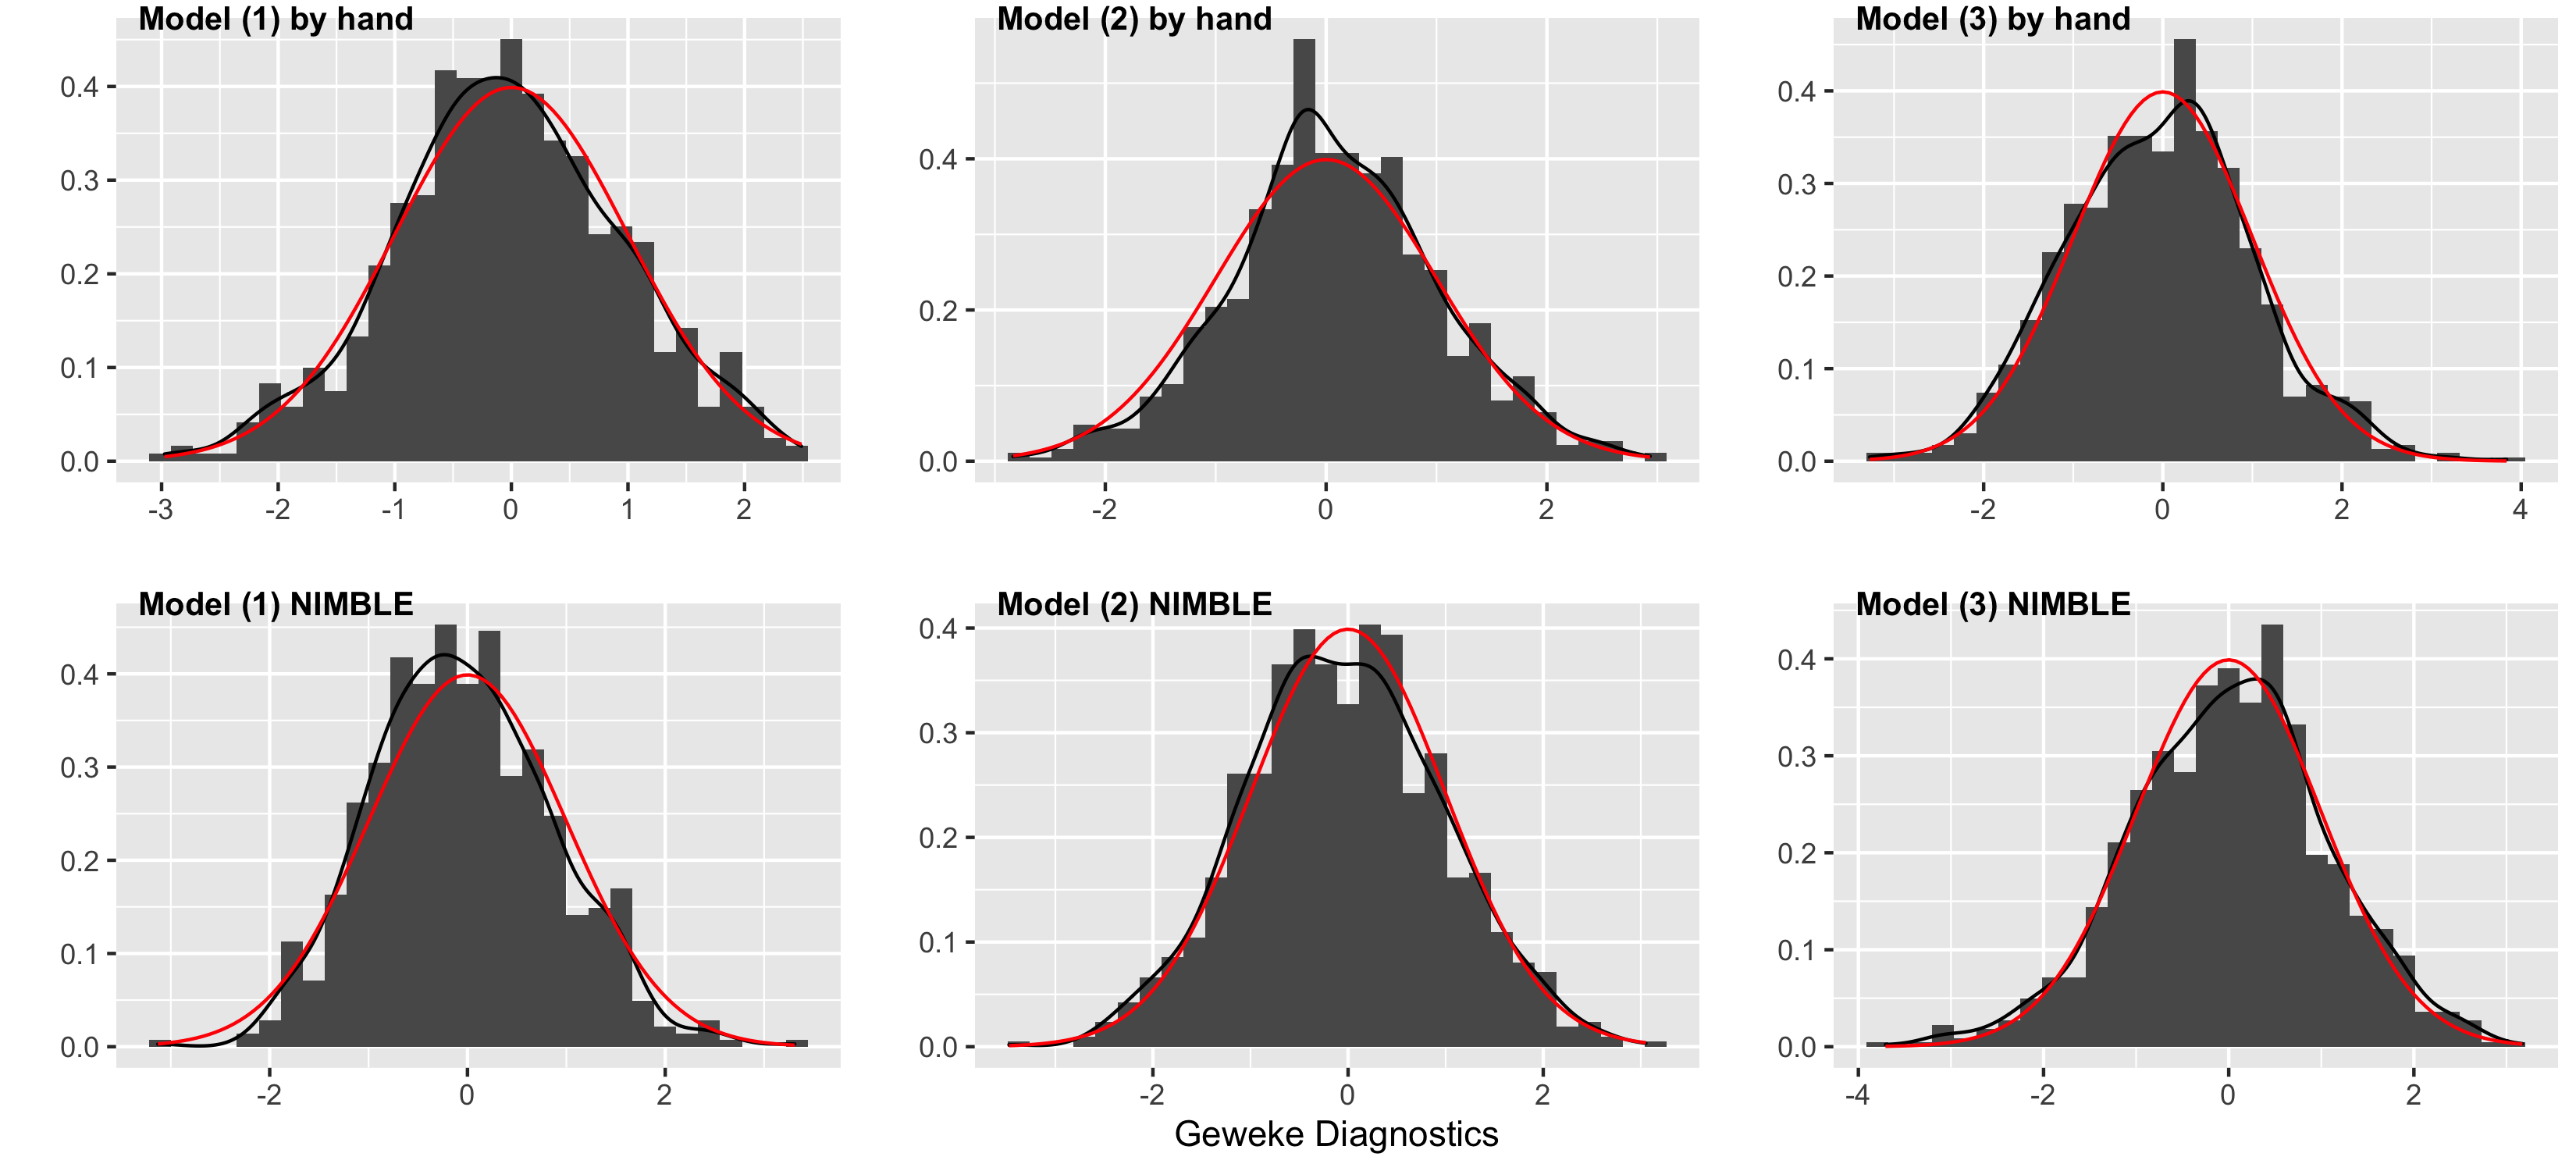
\includegraphics[width=0.8\textwidth]{SemesterProject/geweke_diags.png}
	\caption{Geweke diagnostics for the six model fits given in histogram and KDE (black line) against a standard normal curve (red line). At convergence, Geweke diagnostics are asymptotically N(0,1). }
	\label{fig:geweke}
\end{figure} 


\section{Results}\label{sec:results}

\subsection{Comparison of implementations}

The models fit all estimate a significant number of parameters. Including the estimates of latent variables $Z_{im}$ and $Y_{im}$, Model 1 estimates 34,704 parameters, with a significant amount of shared information bringing the effective number of parameters computed for WAIC calculations down to approximately 2513.1. Model 2 estimates the comparatively less 18,207 parameters ($p_{WAIC}\approx 871.9$). Model 3 estimates three less parameters than Model 2, but has an effective number of parameters closer to Model 1 at around 2058.3. While these parameter counts are high, the data is comparatively larger with 16,800 allele measurements. The way that \citeauthor{efron2016CASI} prepare their data effectively doubles this.

For the same reason that running multiple chains might pollute estimation, comparing the estimates between "by hand" implementations and NIMBLE implementations is not advisable. It is difficult to determine which parameters correspond. When a correspondence is established, it difficult to verify if the true relationship is the one being attributed to it. Because of this issue, establishing if the results of the two implementations agree up to Monte Carlo error is better performed by summarizing the estimates of $Q_i$ than by individual parameter comparison. Using $Q_i$ is preferable since the ordering of parameters is only an issue along one dimension (the different probabilities associated with individual $i$'s ancestry), and a summary can be crafted that is invariant to changes in ordering.

Let $T_i$ represent the ethnicity of individual $i$ as recorded in the data. The summary for comparison of implementations will be the mean distance of all individuals of the same ethnicity from the center of mass in $\mathcal{S}_3$, $\mu_t$, using the estimated $Q_i$ as coordinates. That is the summary quantity for ethnicity $t$, $\phi_t$ is computed as
\begin{equation*}
    \phi_t = \frac{1}{n_t} \sum_{i: T_i = t} \lVert T_i - \mu_t \rVert
\end{equation*}
where $n_t$ is the number of individuals of ethnicity $t$. Figure \ref{fig:model_comp} shows the comparisons.

\begin{figure}[h]
	\centering 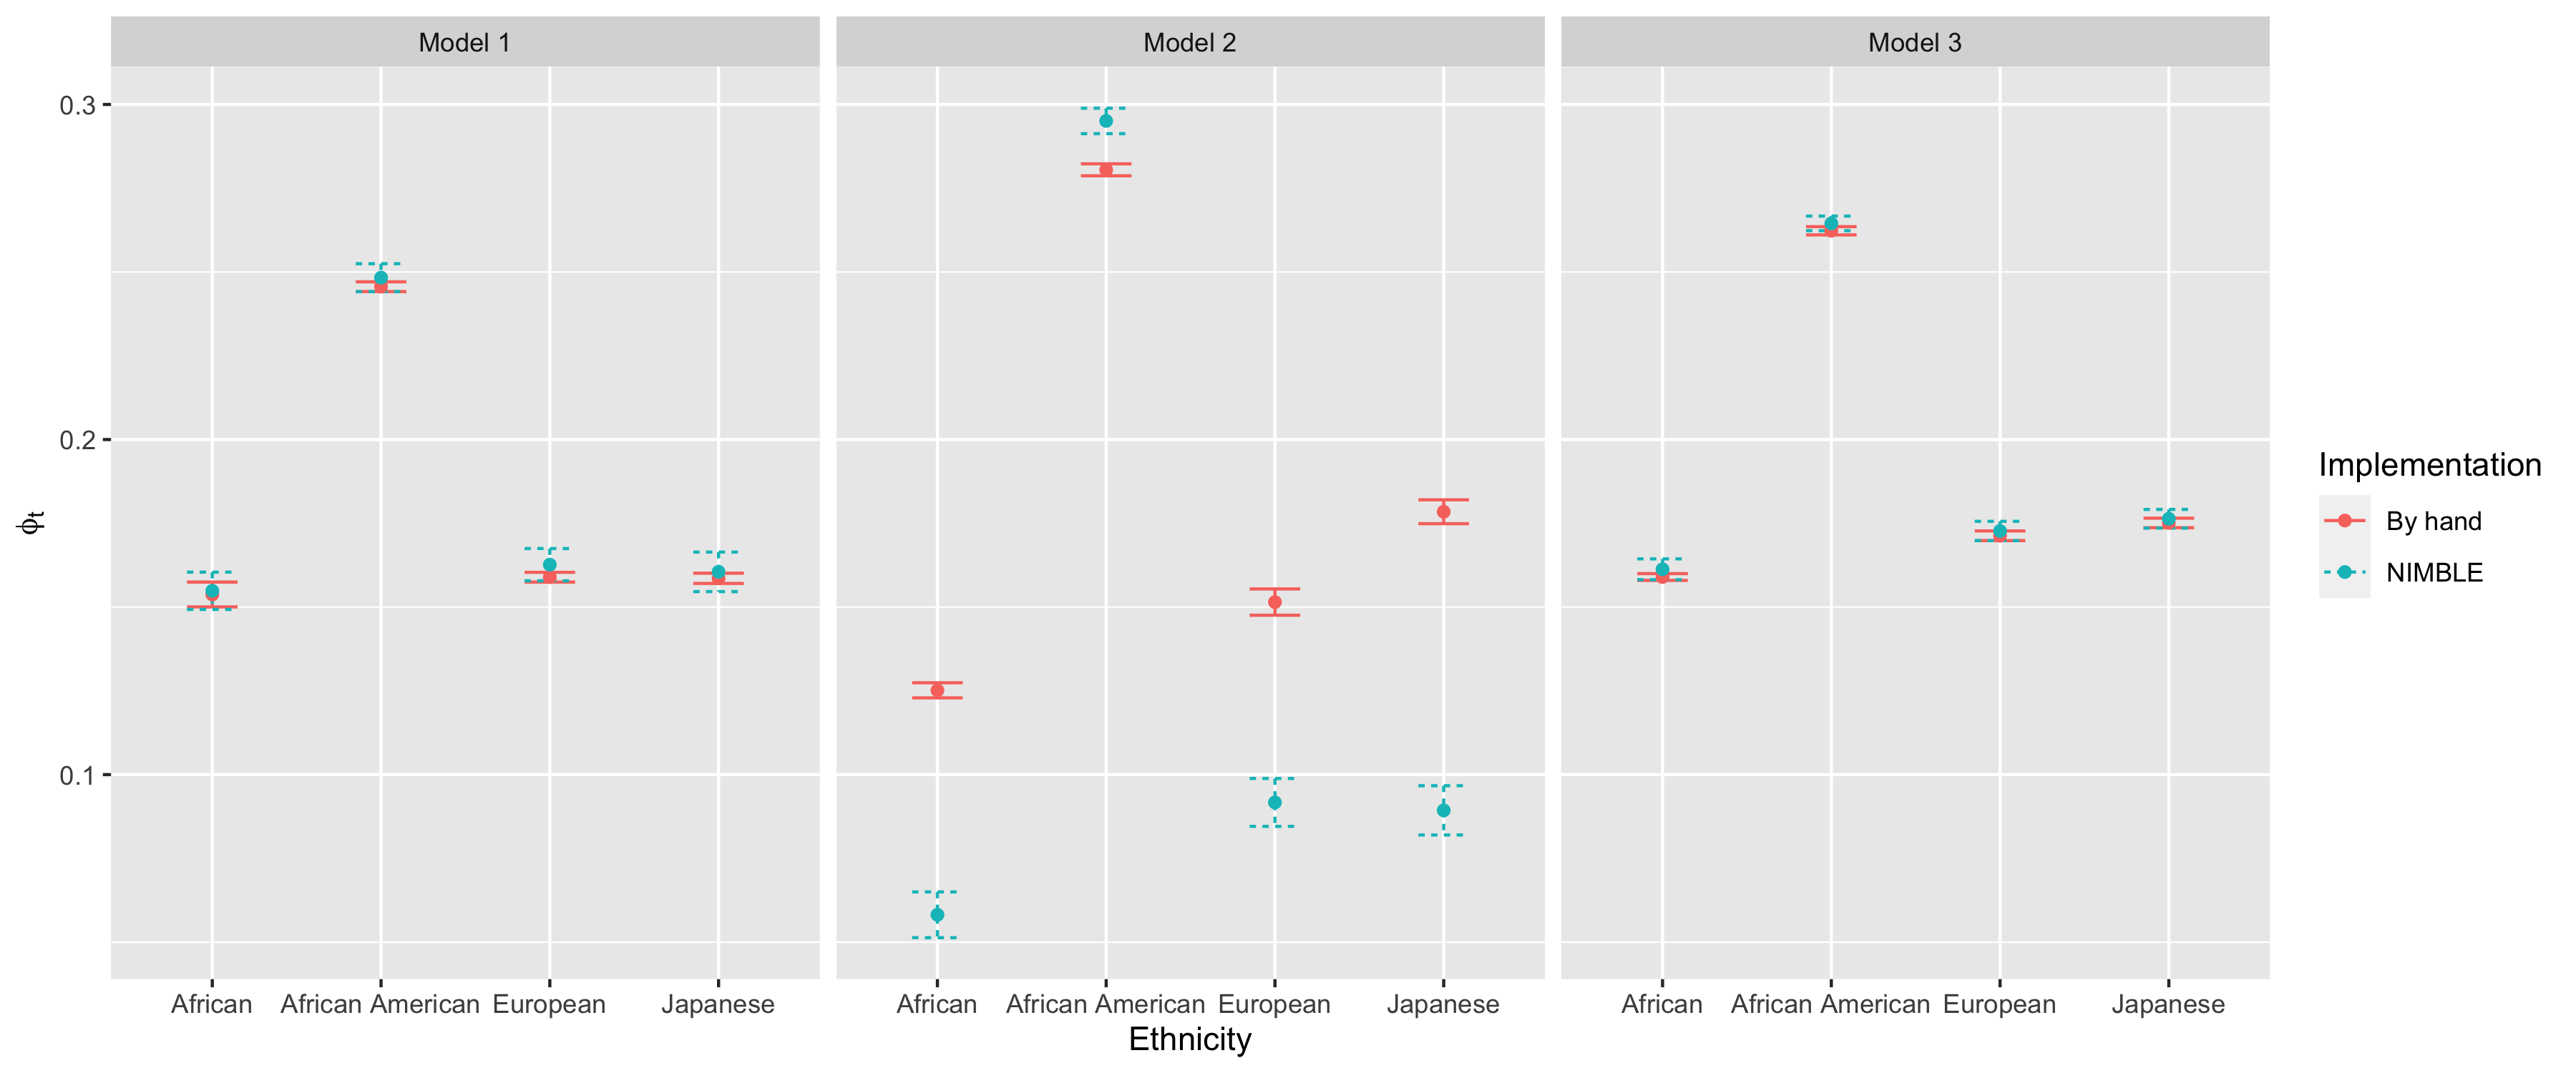
\includegraphics[width=0.8\textwidth]{SemesterProject/model_comp.png}
	\caption{Comparison of implementations of the three models through the summary value $\phi_t$ with Monte Carlo error assessed. Both implementations fit similarly when estimating models 1 and 3. Model 2 displays non-trivial differences between implementations. It is interesting to note that between models 1 and 3, in all cases the point estimates of $\phi_t$ are lower for the model suggested by \citeauthor{efron2016CASI} than for a model that does not reduce uncertainty by arbitrary data preprocessing. These estimates can be interpreted as strength of clustering, with lower values being associated with tighter clustering.}
	\label{fig:model_comp}
\end{figure} 

The discrepancy in the model (2) fits are the consequence of a more interesting phenomenon. Unlike models (1) and (3), model (2) allows for estimation of the shared concentration parameters of the $Q_i$. Further investigation reveals that the two implementations are estimating different values for these parameters (cf. Table \ref{tab:concentration}) while estimating very similar expectations (cf. Table \ref{tab:expectations}). This is likely caused by the tuning parameters of the by-hand Metropolis algorithm being too large to get appropriate acceptance rates when proposing lower values of the concentration parameters. More understanding about the workings of NIMBLE's estimation procedure would be needed to be definitive on this diagnosis.

\begin{table}[]
\centering
\caption{Estimates of concentration hyperparameters. Though inconclusive, the differences in estimates are likely due to differences in estimation procedures as they lead to similar expectations of the elements of $Q_i$ as shown in Table \ref{tab:expectations}.}
\label{tab:concentration}
\begin{tabular}{ccrrrrr}
\hline
Implementation & Quantity  & Estimate & 95\% MC LB & 95\% MC UB & 95\% CrI LB & 95\% CrI UB \\
\hline
By hand        & $\lambda_1$ & 0.261    & 0.190      & 0.346      & 0.260       & 0.261       \\
               & $\lambda_2$ & 0.374    & 0.284      & 0.471      & 0.373       & 0.374       \\
               & $\lambda_3$ & 0.508    & 0.418      & 0.611      & 0.507       & 0.508       \\
               \hline
NIMBLE         & $\lambda_1$ & 0.102    & 0.057      & 0.227      & 0.099       & 0.105       \\
               & $\lambda_2$ & 0.072    & 0.037      & 0.161      & 0.068       & 0.077       \\
               & $\lambda_3$ & 0.059    & 0.029      & 0.150      & 0.057       & 0.062      
\end{tabular}
\end{table}

\begin{table}[]
\centering
\caption{Estimates of the expected value of the elements of $Q_i$ a priori. Though the estimates of the two implementations are not equivalent up to Monte Carlo error, there are certainly strong similarities in reported values. Apparent differences have a likely source in the different estimated values of the concentration parameters reported in Table \ref{tab:concentration}. Note that the estimates in this table provide a good example of the ordering issue discussed in Section \ref{sec:estimation}.} 
\label{tab:expectations}
\begin{tabular}{ccrrrrr}
\hline
Implementation & Quantity    & Estimate & 95\% CrI LB & 95\% CrI UB & 95\% MC LB & 95\% MC UB  \\
\hline
By hand        & $Q_i{[}1{]}$ & 0.228    & 0.227      & 0.229      & 0.171       & 0.299       \\
               & $Q_i{[}2{]}$ & 0.327    & 0.327      & 0.327      & 0.258       & 0.394       \\
               & $Q_i{[}3{]}$ & 0.445    & 0.445      & 0.445      & 0.375       & 0.513       \\
               \hline
NIMBLE         & $Q_i{[}1{]}$ & 0.450    & 0.450      & 0.451      & 0.370       & 0.524       \\
               & $Q_i{[}2{]}$ & 0.306    & 0.306      & 0.306      & 0.242       & 0.374       \\
               & $Q_i{[}3{]}$ & 0.243    & 0.243      & 0.244      & 0.187       & 0.316      
\end{tabular}
\end{table}

\subsection{Discussion of model implications}

The three models fit represent different assumptions about the data. Model (1) asserts that the generative model is a valid representation. Models (1) and (2) assume a priori that the density of $Q_i$ is uniformly distributed, while model (3) assumes uniformity in expectation over the hyperprior. These models allow for insight into first, if the generative model leads to the same conclusions as a model without and second, if changing concentration parameters changes inference on admixture. Our motivating question is such that changing the number of latent populations should not be considered as part of a sensitivity analysis. Figure 3 visualizes admixture from four different model fits. 

\begin{figure}[h]
  \begin{subfigure}[t]{.4\textwidth}
    \centering
    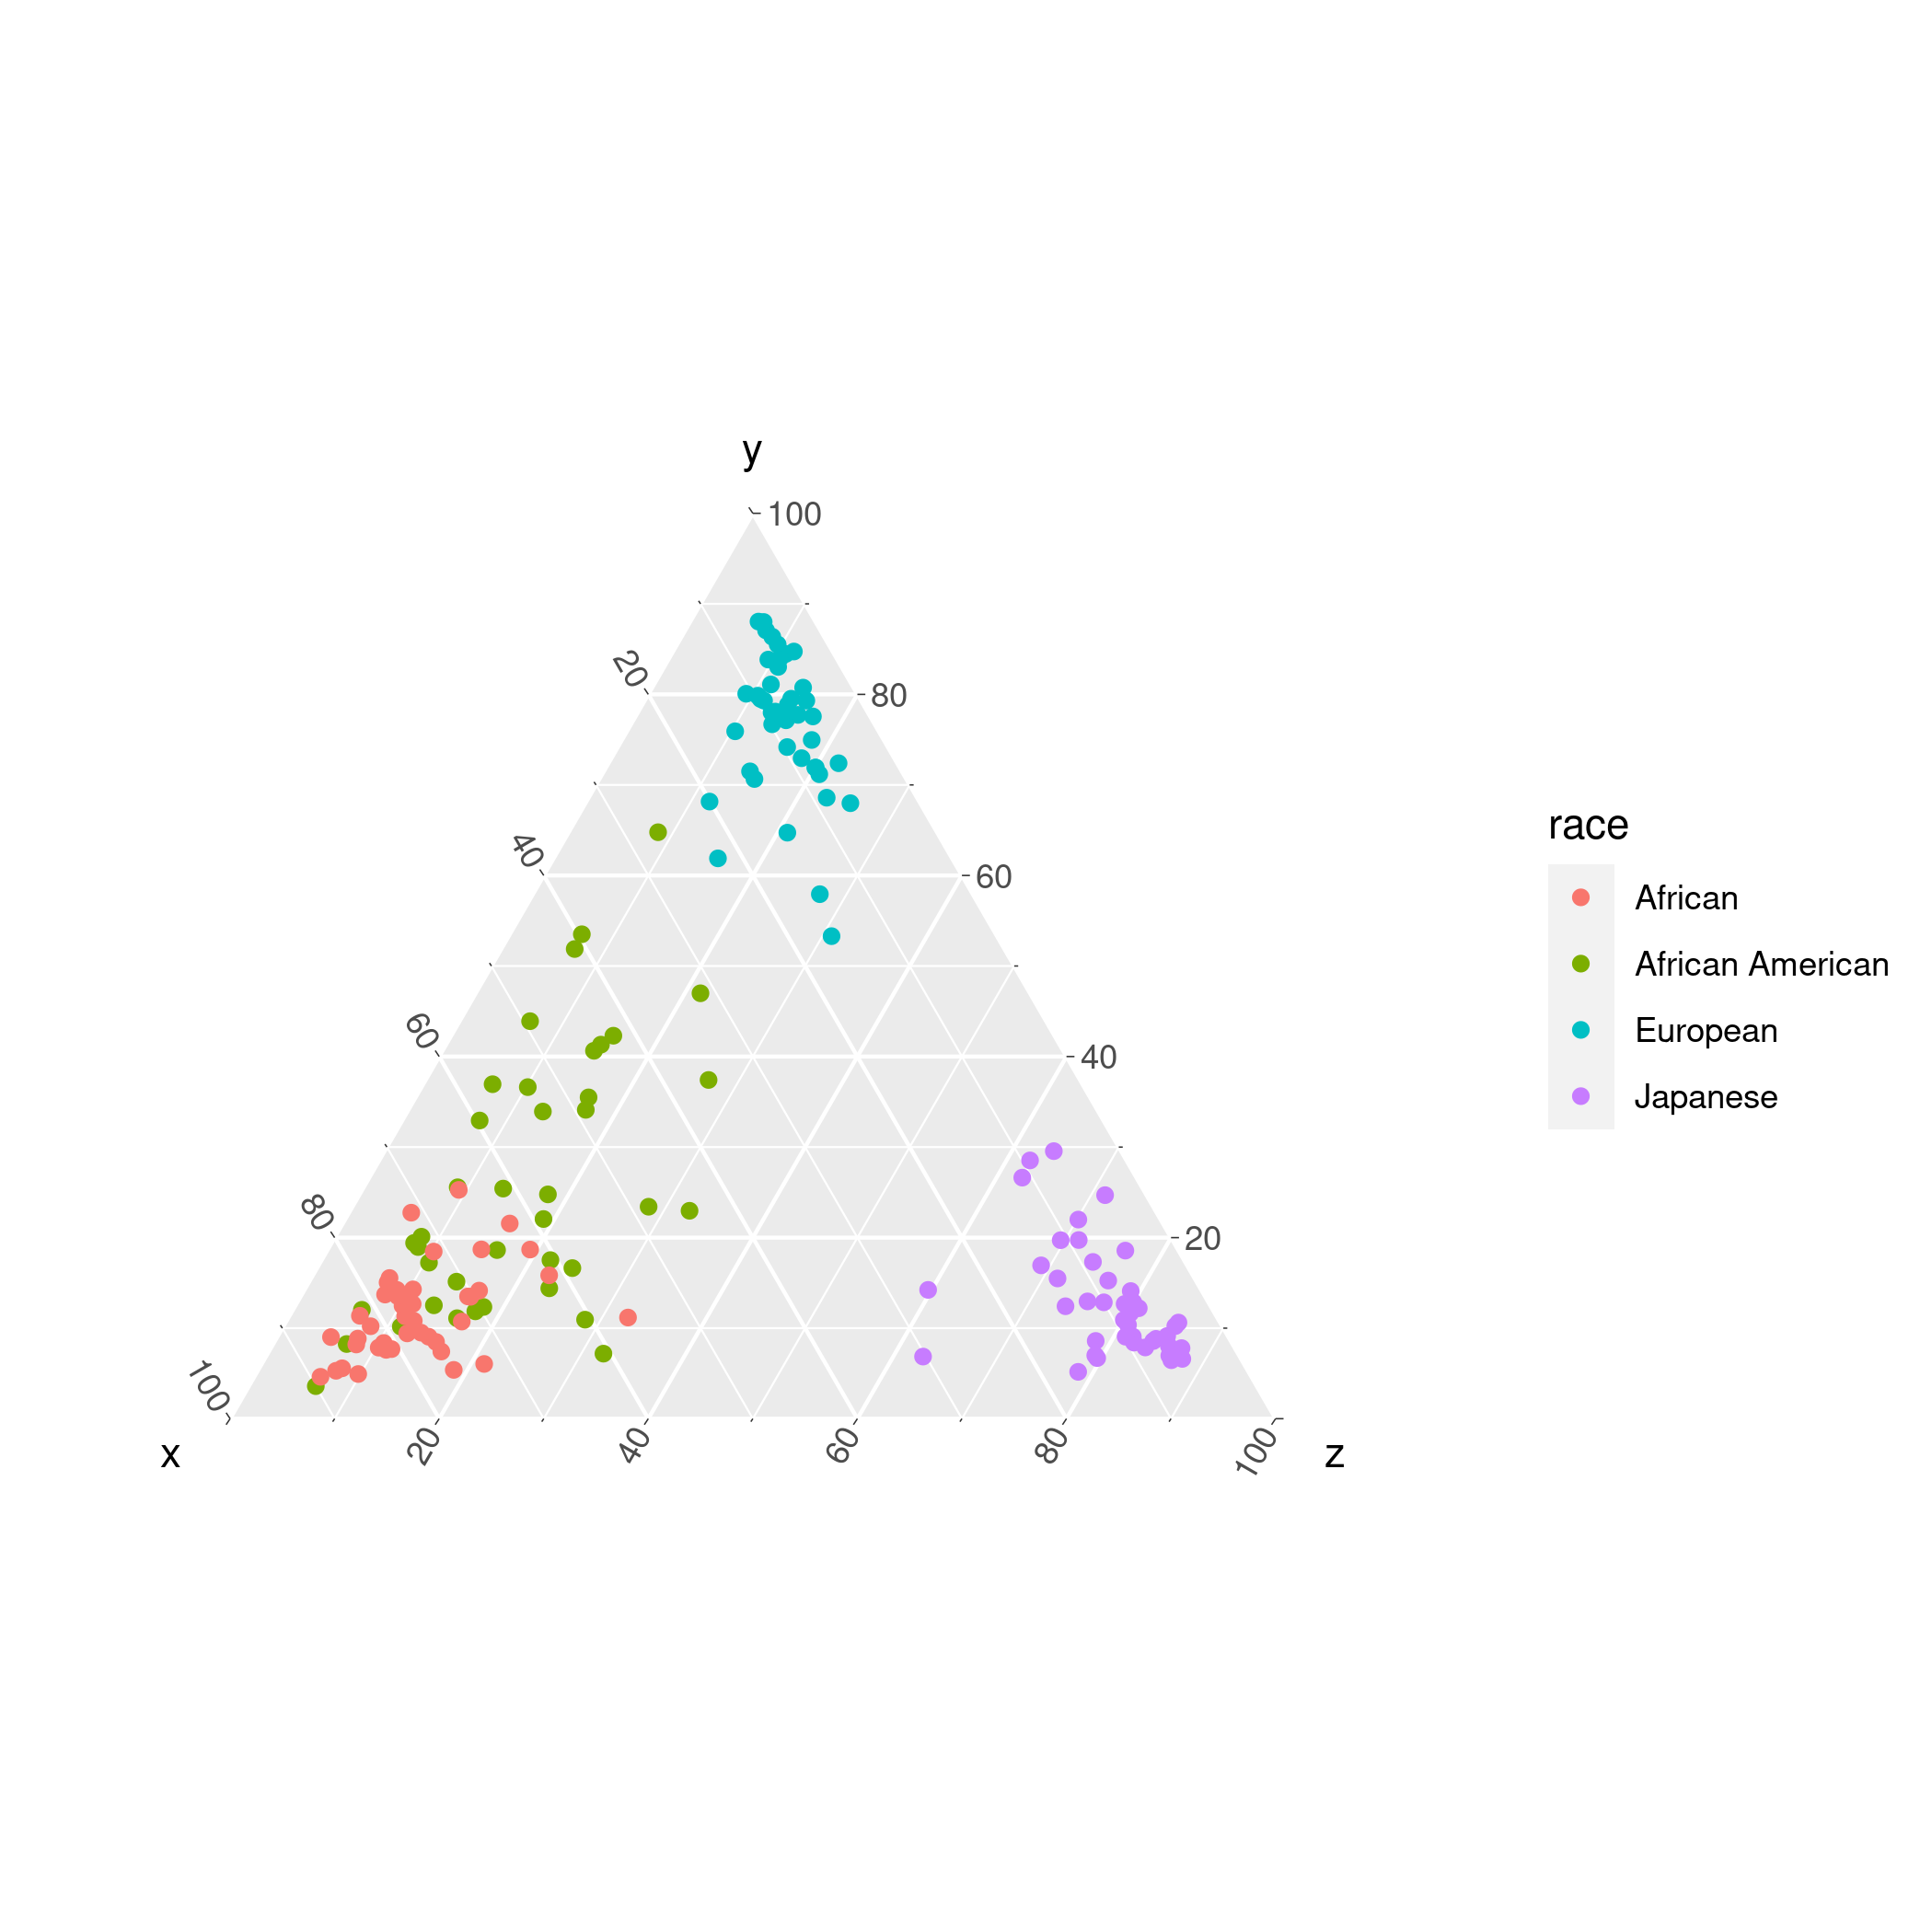
\includegraphics[width=\linewidth]{SemesterProject/haplo_tern_mod1.png}
    \caption{\textbf{Model (1)}: Ternary plot of estimated $Q_i$ of the model proposed by \citeauthor{efron2016CASI}, $\lambda_Q = (1, 1, 1)$.}
  \end{subfigure}
  \hfill
  \begin{subfigure}[t]{.4\textwidth}
    \centering
    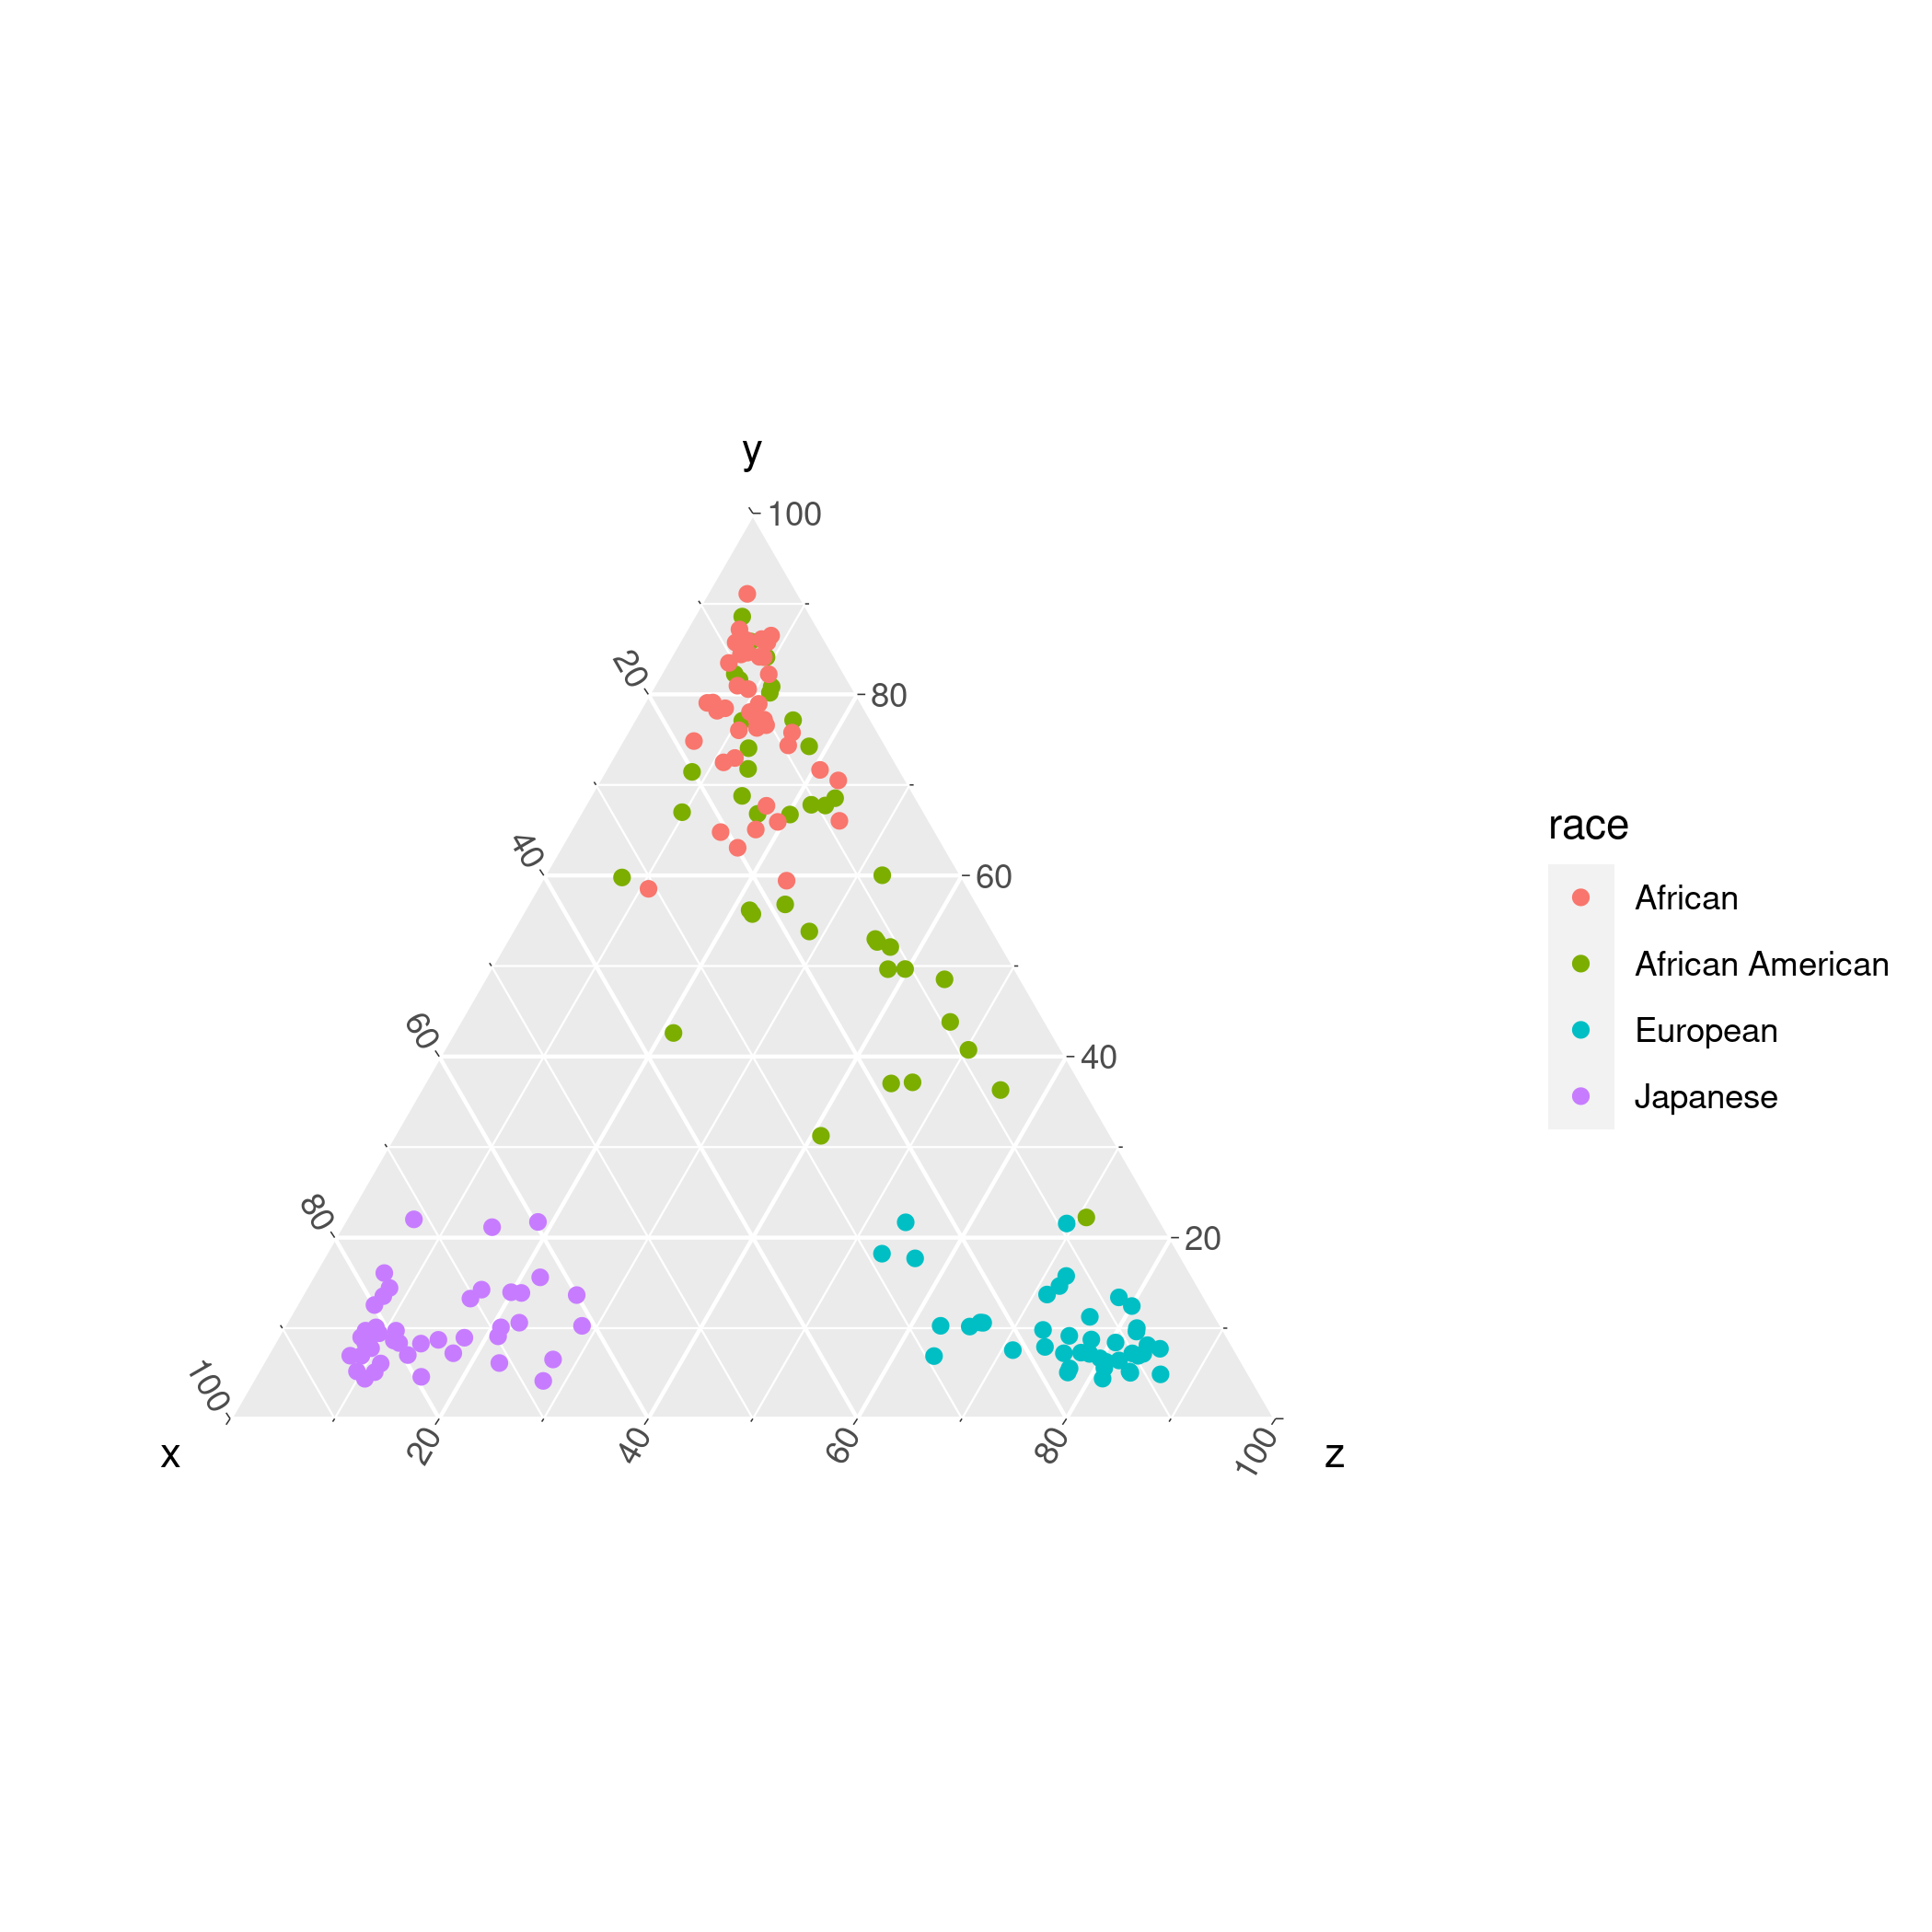
\includegraphics[width=\linewidth]{SemesterProject/haplo_tern_mod3.png}
    \caption{\textbf{Model (3)}: Ternary plot of estimated $Q_i$ of model with same priors as \citeauthor{efron2016CASI} but with no use of generative model, $\lambda_Q = (1, 1, 1)$.}
  \end{subfigure}

  \medskip

  \begin{subfigure}[t]{.4\textwidth}
    \centering
    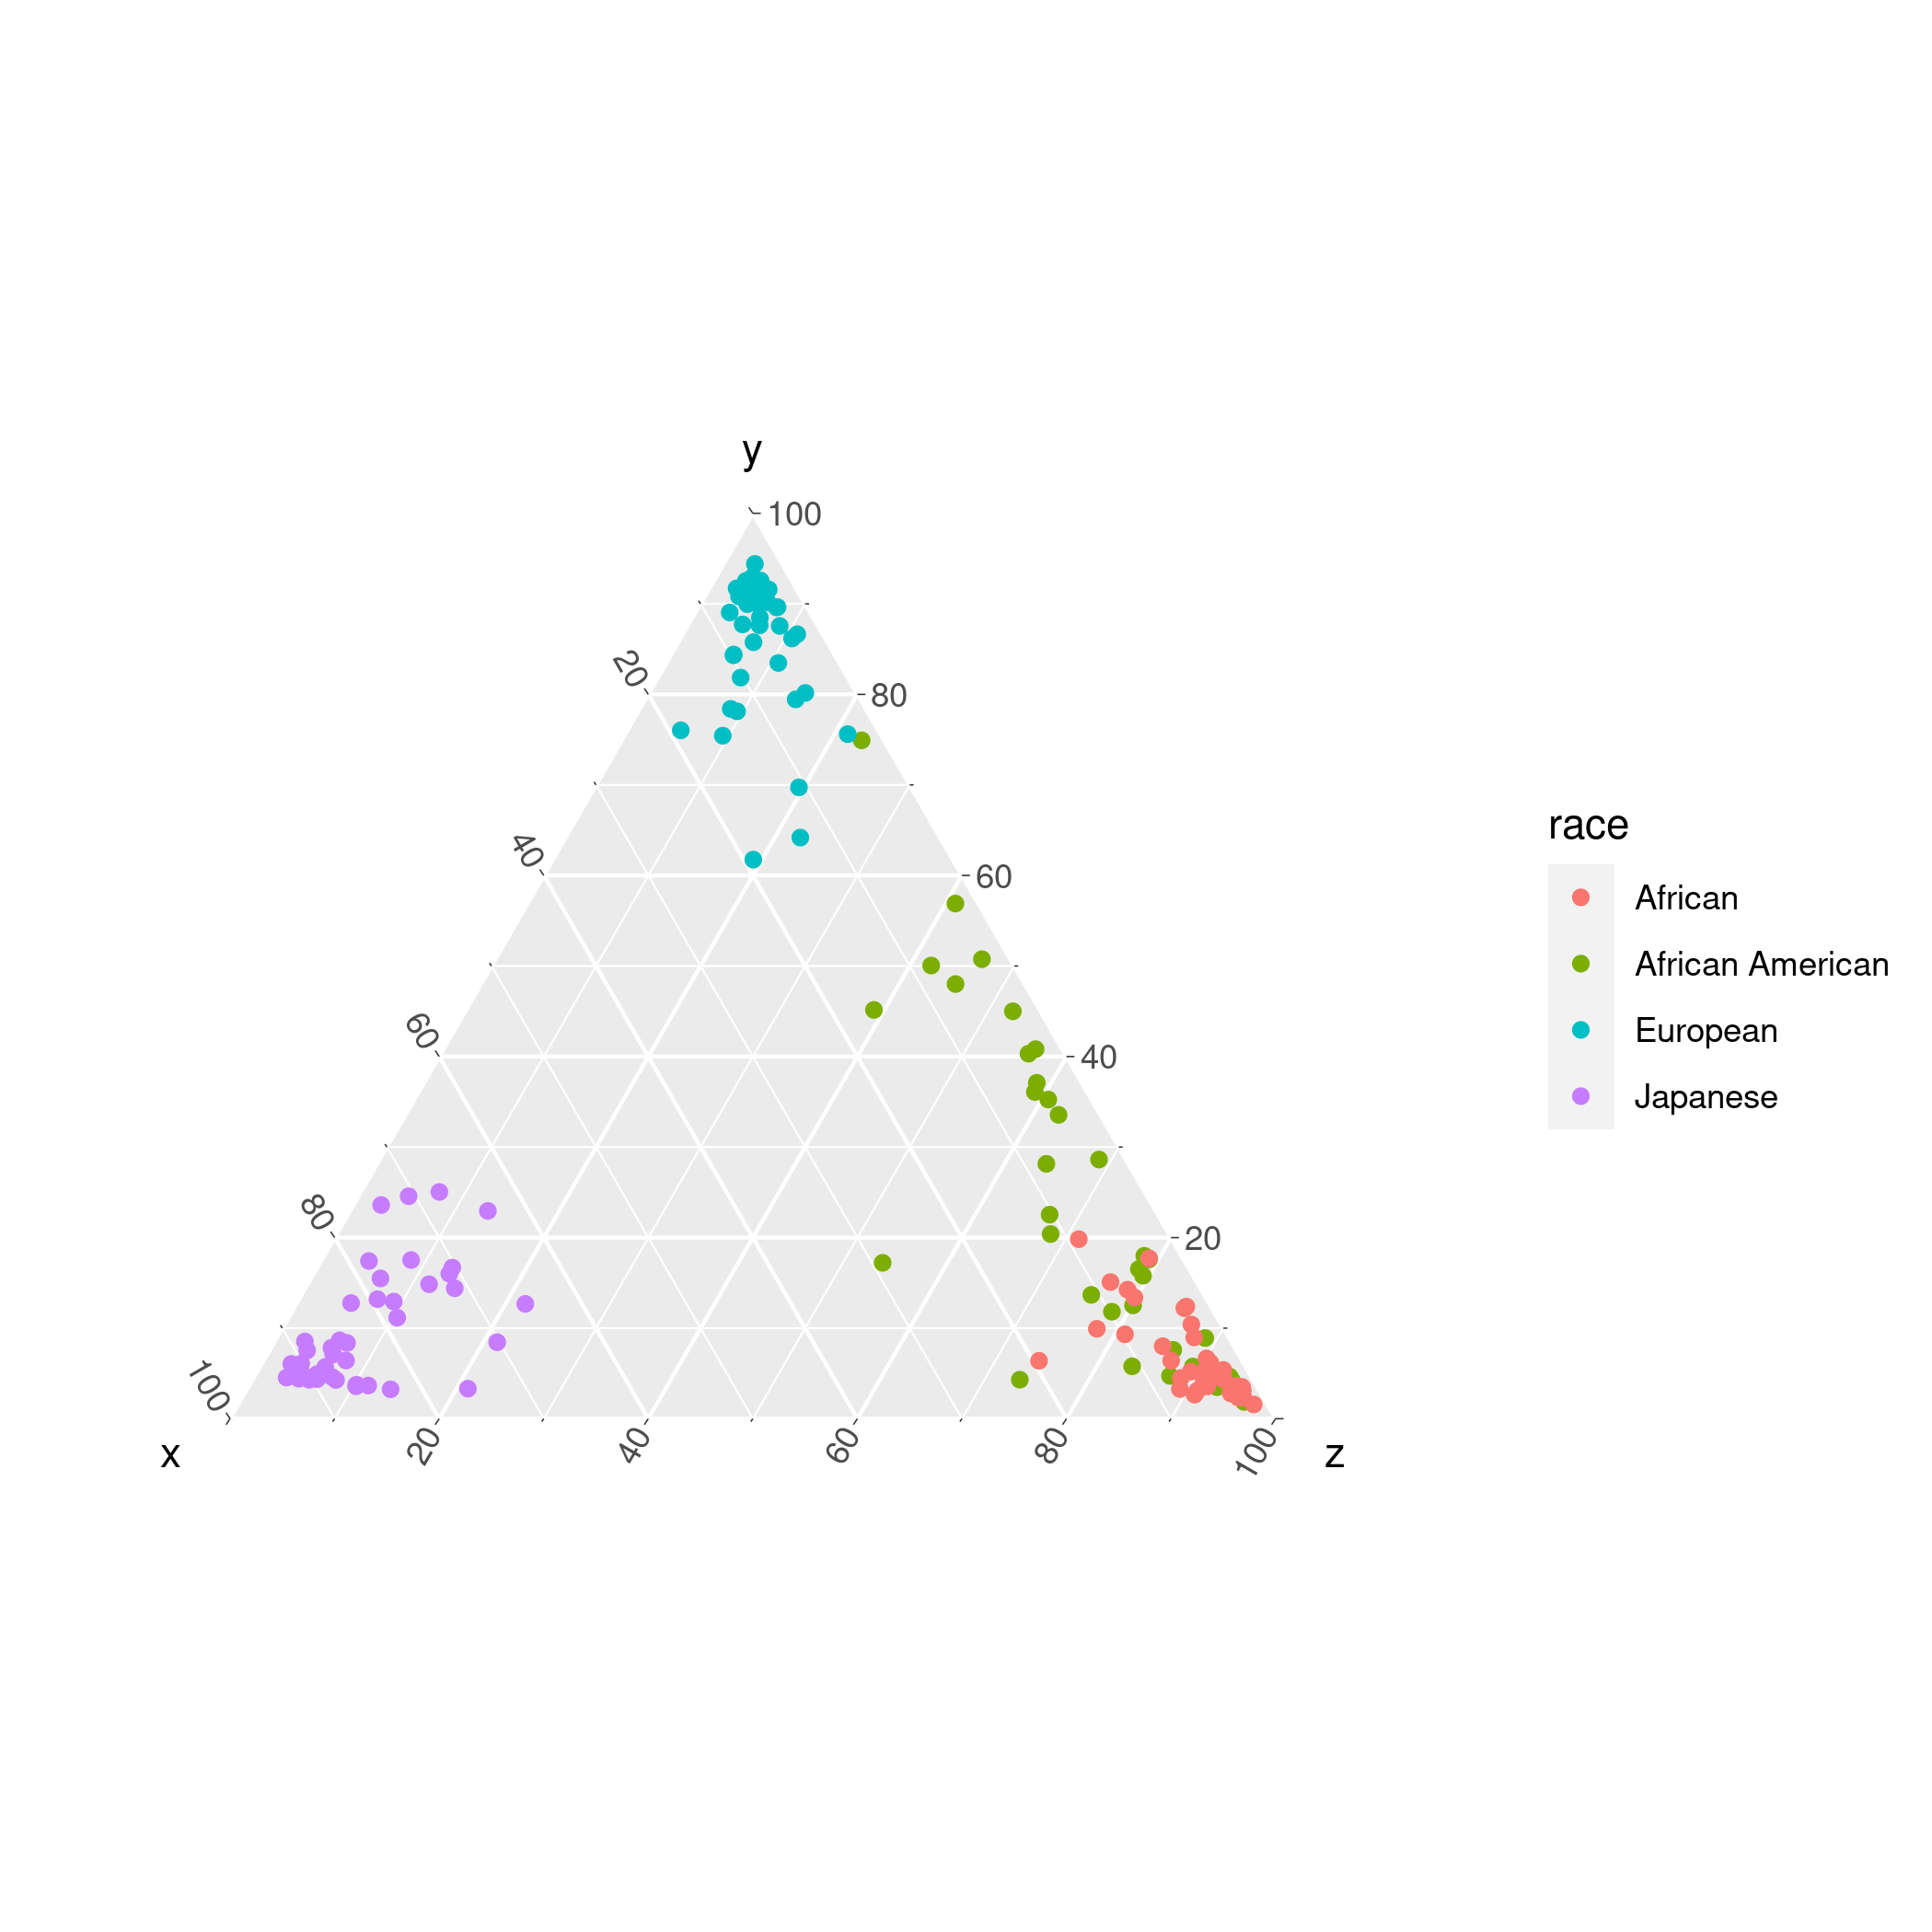
\includegraphics[width=\linewidth]{SemesterProject/haplo_tern_mod3BH.png}
    \caption{\textbf{Model (3) fit by hand}: Ternary plot of estimated $Q_i$ of model with independent gamma priors on $\lambda_Q$, $\hat{\lambda}^{\text{MSE}}_Q = (0.261, 0.374, 0.508)$.}
  \end{subfigure}
  \hfill
  \begin{subfigure}[t]{.4\textwidth}
    \centering
    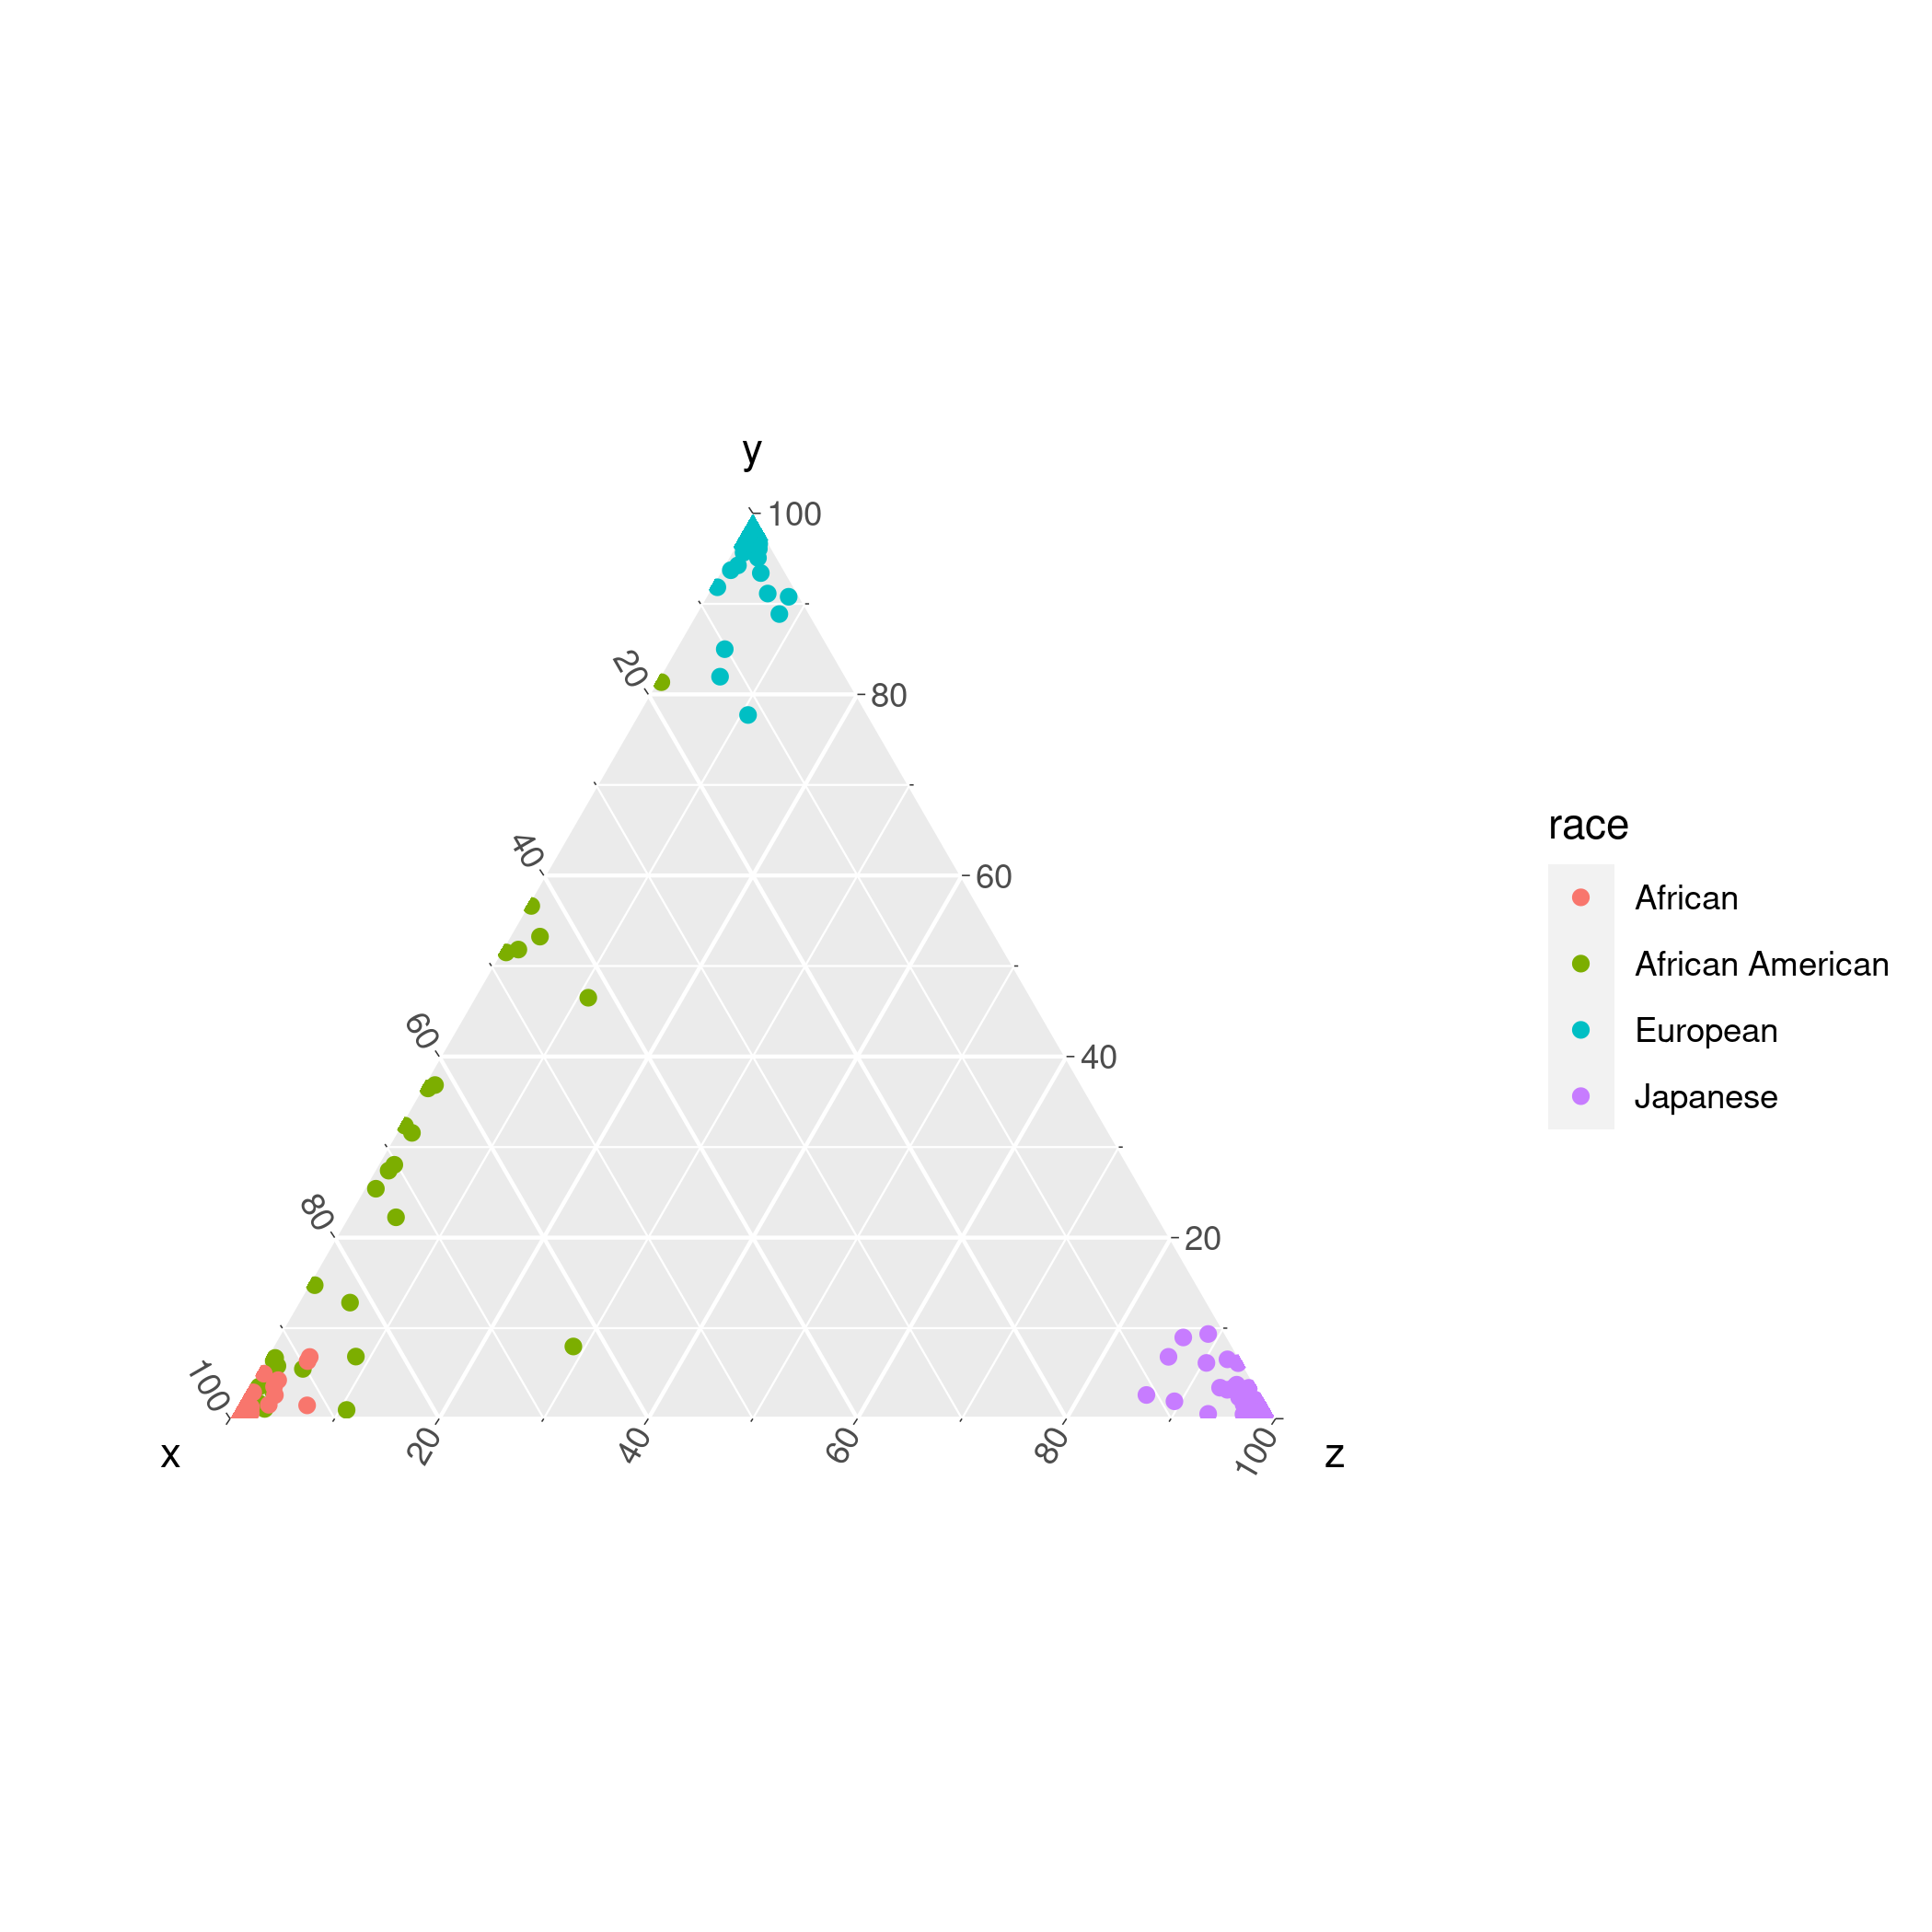
\includegraphics[width=\linewidth]{SemesterProject/haplo_tern_mod3NIMBLE.png}
    \caption{\textbf{Model (3) fit by NIMBLE}: Ternary plot of estimated $Q_i$ of model with independent gamma priors on $\lambda_Q$, $\hat{\lambda}^{\text{MSE}}_Q = (0.102, 0.072, 0.059)$.}
  \end{subfigure}
  \caption{Ternary plots displaying fits of various models, each expressing different assumptions about the data. On display is the permutation of the group orderings, seen by the clustering of ethnicities into different corners by different models. Comparing (a) to (b) shows visibly tighter clustering of ethnicities under Model (1) than under Model (3), a different view of the phenomenon identified in Figure \ref{fig:model_comp}. Putting gamma priors on the $\lambda_Q$ hyperparameters results in estimation that puts more density around the edges of the plotted region, lower values being associated with less density concentrated in the center. All models give similar inference about the admixture of the \texttt{African American} ethnicity, though individual-level inference varies.}
  \label{fig:results}
\end{figure}

A comparison of Figures 3 (a) and (b) shows only minor, though visible, effects of the generative model. As expected from Figure \ref{fig:model_comp}, using the generative model encourages slightly tighter intra-group clustering than a model of the data without the extra step. Thus, while models (1) and (3) are similarly reasonable, it does further underscore the question of expediency as it relates to using the generative model in the context of the likelihood function of the data. By this analysis, I would say that the model proposed by \citeauthor{efron2016CASI} is a benign theoretical misstep. Their approach does not lead to different conclusions about admixture, a mark both for and against it.

The effect of decreased concentration parameters, seen by including Figures 3 (c) and (d) in the comparison, further tightens clustering by pushing density towards the edges of the plotted region in the prior and posterior. It would be trivial to fit a model with increased concentration parameters; the observations would remain in the same relative positions but be compressed towards whatever point the prior concentrations center on. By inspection we see that small concentrations emphasize the placement of \texttt{African American} individuals along the \texttt{African-European} spectrum while de-emphasizing the measured influence of \texttt{Japanese} inheritancy. Thus, dogmatism about the concentration parameters will influence subjective interpretation of the cardinal influence of the various populations. However, since the meaning of each concentration parameter is uncertain prior to model fitting, it is thought highly improbable that the parameters could be tweak to change the ordinal influences. A simulation study is beyond the scope of this assignment, but the it is asserted that the influence of \texttt{African} and \texttt{European} ancestry on \texttt{African American} individuals will always be found to exceed that of the \texttt{Japanese} population in any model that finds meaningful clusters.

\section{Comparison to non-Bayesian Latent Class Model}\label{sec:frequentist}

A non-Bayesian model that can estimate similar probabilities as those represented in $Q_i$ is a latent class model. A latent class model has utility in statistical applications where inference centers on an unobserved categorical variable and manifest variables are likewise categorical. Latent classes are initialized, and then the model is fit via the EM algorithm or anther optimization, such as Newton-Raphson. Expected cell counts of the joint contingency table of latent and manifest variables are estimated using a log linear model. Conditional probabilities of an individual being a member of class a certain $Z$ given their manifest variables can be calculated from the application of basic probability rules on the fitted values of the model after convergence is achieved. For more detail, see \cite{agresti2003CDA}.

Fitting a log-linear model is made more difficult when cell counts are small. In the context of the population admixture question, this means that a latent class model will reach a point that it fails to be useful once a certain number of SNP loci are included as explanatory variables. This can be remedied using highly subjective variable selection. The latent variables make objective algorithmic approaches to variable selection untenable. Figure \ref{fig:non-bayesian} shows two latent class models fit to the data.

\begin{figure}[h]
    \centering
    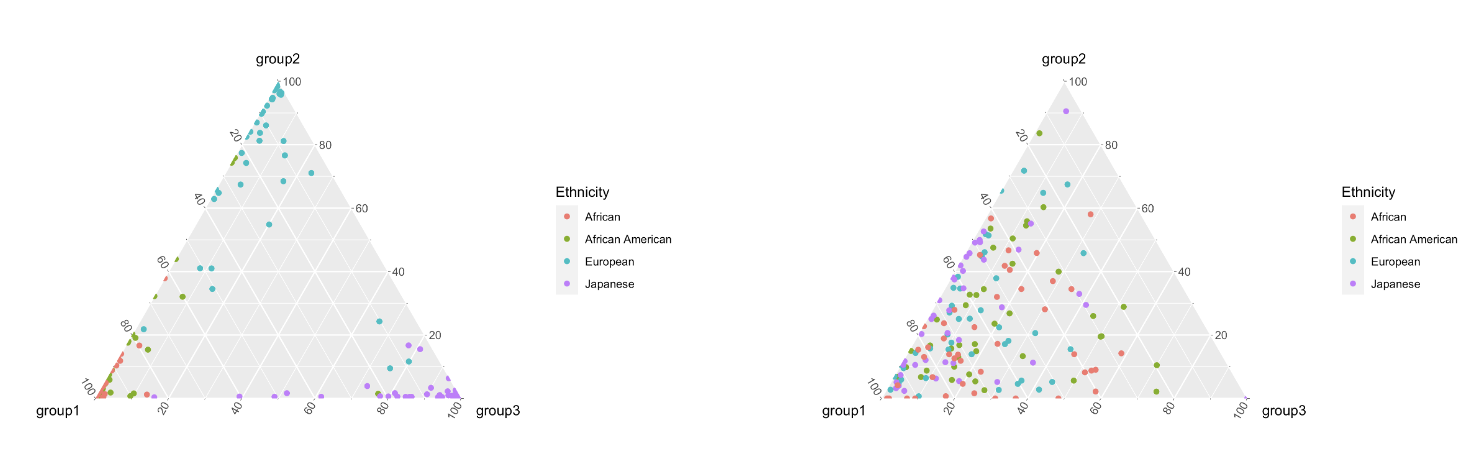
\includegraphics[width=0.8\textwidth]{SemesterProject/nonbayesian_method.png}
    \caption{Estimation of admixture using a latent class model fit with 9 carefully selected SNP loci (left) and all SNP loci with empirical variance greater than 0 (right). Poor fit is to be expected with a sparse contingency table like the kind this data creates. Better clustering than this can be achieved with thoughtful variable selection, though this is a highly subjective process and the Bayesian method requires less input from the modeler.}
    \label{fig:non-bayesian}
\end{figure}

A Bayesian model is better suited to this analysis because of the ability to better borrow strength across individuals and SNP loci. The Bayesian approach is simpler to implement and understand, and it results in richer clustering while also providing a stronger degree of separation between the ethnicities. The non-Bayesian latent class model is severely limited by comparison.

% bibliography section
\bibliographystyle{plainnat}
\bibliography{project}

\end{document}
